\chapter{基于 OOK 调制的 NLOS OCC 系统}
\section{系统概述}
NLOS OCC系统作为作为NLOS IS-VLP系统的一个核心模块,在接收端,对LED进行调制驱动,在接收端,对接收到的光信号进行解调解码,实现对LED的位置信息进行接收。基于上一章节的基础理论,这一章节将详细阐述如何设计一个基于OOK 调制的 NLOS OCC 系统。主要包括NLOS OCC信号恢复模型、系统硬件设计和接收端信号恢复。需要注意的是,本章内容将作为本文所提出的NLOS IS-VLP系统的一个主要模块,在后续章节中将默认已经通过本章节的NLOS OCC系统实现对LED坐标的接收而不再单独进行叙述其过程。

\section{NLOS OCC 信号恢复模型}
在NLOS OCC信道理论的基础上,本系统给出了一个NLOS OCC 信号恢复模型,它将为NLOS OCC系统信号恢复提供理论支持。与基于PD的VLC系统不同,OCC系统中,接收端相机的一个像素是光信号接收的最小单位。所以,本系统更多的考虑如何计算任意一个像素的灰度值。把环境光考虑在内,像素$(u,v)$的辐射强度可以表示为:
\begin{equation} \label{ruvt}
r(u,v,t) = a(u,v)+l(u,v)s(t),
\end{equation}
其中$a(u, v)$是环境光的辐射强度,$l(u, v)$是在没有调制信号下的像素$(u,v)$区域内LED辐射强度的积分,$s(t)$是调制信号。因此,OCC系统的成像模型可以定义为:
\begin{equation}\label{iuv}
i(u,v) = k\int_{-\infty }^{\infty } r(u,v,t)f(u,v,t)dt+n(u,v)
\end{equation}
其中,$k$是将辐射度转换为像素灰度值的传感器增益,$n(u,v)$是图像噪声。注意,(1)图像噪声是由外部来源引起的图像质量的退化,在图像采集、编码、传输和处理等每一个步骤中始终存在;(2)图像噪声会随着图像亮度、颜色动态随机变化,会随着相机的感光度、快门时间、温度而增加。
假设$f(u,v,t)$是相机的曝光函数,由于CMOS相机的卷帘快门特性,$f(u,v,t)$可以表示为与像素行$v$相关的一个矩形时间窗函数,由以下公式给出:
\begin{equation}\label{fuvt}
f(u,v,t)=e(t_{v}-t)
\end{equation}
其中$e(t_v - t)$是一个快门函数,定义为:
\begin{equation}\label{etv-t}
e(t_{v}-t)=\begin{cases}
   1,t\in(t_{v}-\Delta t, t_{v})\\
  0,t\notin (t_{v}-\Delta t, t_{v})	
\end{cases}
\end{equation}
其中$\Delta t $是每行像素的曝光时间,$t_v$是第$v$行初始曝光时间,根据公式(\ref{fuvt}),公式(\ref{iuv})可以改写为
\begin{equation}\label{iuv+}
i(u,v) = k\Delta ta(u,v)+kl(u,v)g(v)+n(u,v)
\end{equation}
其中$g(v)$是快门函数$e(t_v-t)$和信号函数$s(t)$的卷积,可以表示为:
\begin{equation}\label{gv}
g(v)=\int_{-\infty }^{\infty } e(t_{v}-t)s(t)dt=e*s( t_{v})=e*s( v\Delta t )
\end{equation}
众所周知,$k \Delta t a(u,v)$是环境光分量,是一个常数,当LED关闭时,可以得到:
\begin{equation}\label{iauv}
i_{a}(u,v) = k\Delta t a(u,v)+n(u,v)
\end{equation}
注意,只要图像具有较高的信噪比,那么$n(u,v)$的影响就可以被忽略。在这里,使用帧减法来过滤公式(\ref{iuv+})中的环境光成分,即噪声,因此有:
\begin{equation}\label{$delta$iuv}
  \Delta i(u,v) = kl(u,v)g(v)
  \end{equation}
先对公式(\ref{$delta$iuv})进行傅里叶变换,然后对每一行的像素值进行求和后,将得到以下结果:
  \begin{equation}\label{Iw}
  I(\omega )=L(\omega )*(E(\omega )S(\omega ))
  \end{equation}
注意,$\Delta t $可以通过改变快门时间来改变,这就意味着可以选择性的调整每一行像素的曝光时间。当选择两个不同的快门时间捕获两张图片,由于$l(u,v)$与时间无关,可以得到以下的关系:
  \begin{equation}\label{I1E2Sw}
  I_{1}(\omega )*(E_{2}(\omega )S(\omega ))-I_{2}(\omega )*(E_{1}(\omega )S(\omega ))=0
  \end{equation}
可以把时间信号$s(t)$看成是由一个小的、离散的时间频率集$Ω=[w_1,w_2,...,w_m]$组成。因此$\vec{I_1}$ 可以被视为一个矢量,它由$I_{1}(ω)$的不同频率分量组成,同样的,$\vec{I_2}$,$\vec{E_1}$,$\vec{E_2}$,$\vec{S}$也是如此。方程(\ref{I1E2Sw})可以用矩阵形式表示为:
  \begin{equation}\label{I1E2-I2E1}
  (\mathbf{I_{1}E_{2}} -\mathbf{I_{2}E_{1}} )\vec{S}=0
  \end{equation}
 其中$\mathbf{I_1}$和$\mathbf{I_2}$是由$\vec{I_1}$,$\vec{I_2}$决定的T型矩阵。$\mathbf{E_1}$和$\mathbf{E_2}$是由$\vec{E_1}$,$\vec{E_2}$决定的对角矩阵。通过求解线性方程组(\ref{I1E2-I2E1})来得到$\vec{S}$。图\ref{fig:signalrecovery}显示了NLOS OCC系统中信号恢复的整个过程,即信号恢复模型。
\begin{figure*}[!t]
  \centering
  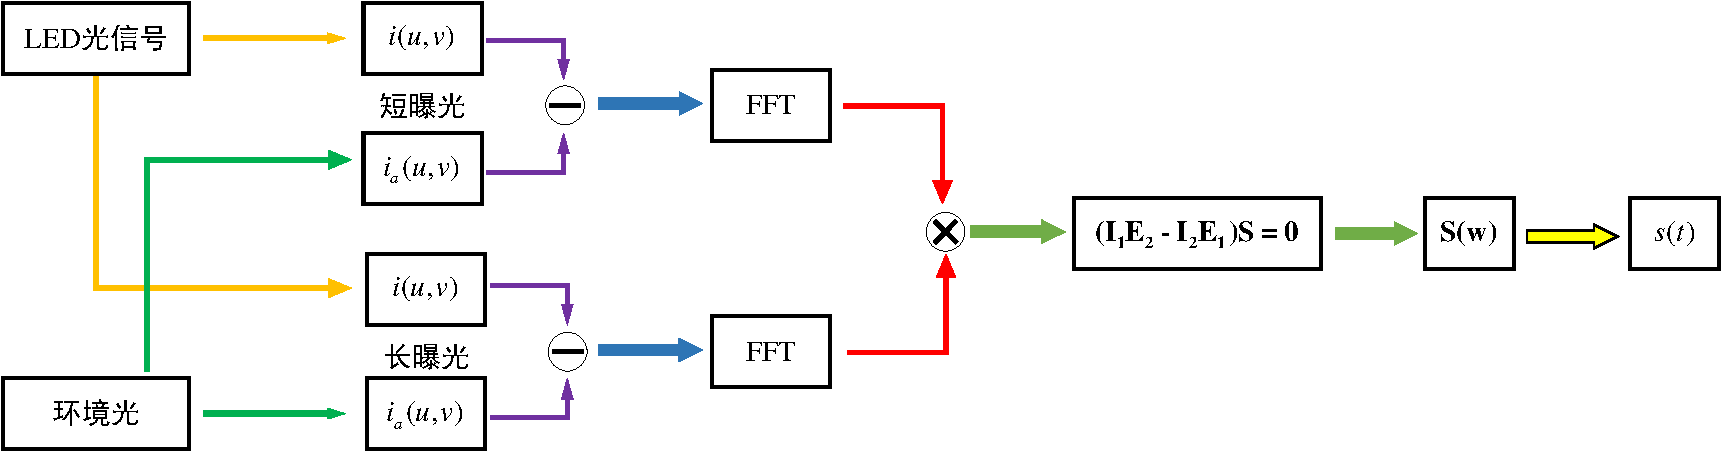
\includegraphics[width=\linewidth]{FIG/signalrecovery.pdf}
  \caption{NLOS OCC系统的信号恢复模型}
  \label{fig:signalrecovery}
\end{figure*}


\section{系统设计}
前面的内容介绍了NLOS OCC系统的基本理论和方法,在这里给出最简单的使用单个LED的基于OOK调制的NLOS OCC系统设计方法,包括硬件系统设计和接收端信号恢复方法,整个NLOS OCC系统的流程图如图\ref{fig:OOK NLOS OCC}所示。需要注意的是由于OOK调制的调制信号没有偏置电压,信号函数是一个方波,由此可以对信号恢复模型进行简化,大部分时候使用直接强度检测的方式进行信号恢复。
\begin{figure*}[!htbp]
  \centering
  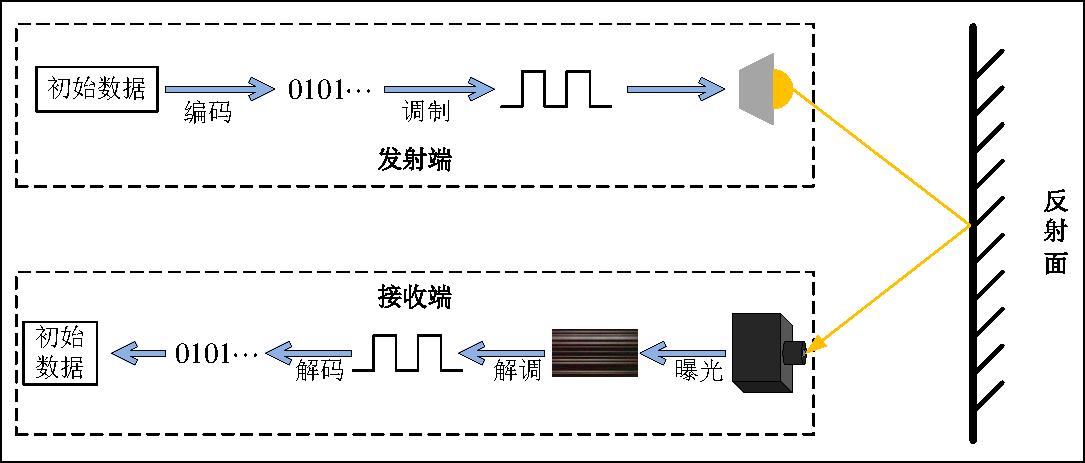
\includegraphics[width=\linewidth]{FIG/OOK NLOS OCC.pdf}
  \caption{基于 OOK 调制的 NLOS OCC 系统流程图}
  \label{fig:OOK NLOS OCC}
\end{figure*}

\subsection{硬件系统设计}
整个硬件系统非常的简单,首先是发射端,一个LED被放置在距离地面1.96米高的天花板上,通过直流电源为其供电。首先将原始数据进行二进制化,然后对二进制数据使用曼彻斯特编码。然后选择一个STM32微控制器单元(MCU)将编码按照OOK调制,“0”输出低电平,“1”输出高电平,MCU输出的频率为5 kHz。输出的电压信号将用来控制一个驱动器,高电平使其出口节点导通,低电平使其出口节点断开。将这一对节点串联在直流电源和LED的中间从而控制LED的亮灭,由此来控制LED的发光强度。需要注意的是,由于相机每一帧图像之间有帧间间隙,因此接收端对发射端时间信号的采样并不是按照一定的时间间隔连续不间断进行的。因此,为了考虑接收端信号恢复的完整性,一般有两种思路。第一种思路是重传机制,考虑将需要发送的信号分成多个连续的子包,在每一个子包的帧头有编号,当在帧间间隙时间丢失了某个子包或者接收不完整,可以考虑通过上行链路给接收端发送重传指令,然而在VLP系统中,经常都是单工模式,因此这种思路一般很少用。第二种方法是考虑在一帧图像里面能够最少两次完整的发送数据包,这样接受保证在接收端至少完整的接收到一个数据包 。这种方式需要牺牲一定的速率,并且要考虑相机帧率和发射端的频率匹配。在VLP系统中,由于发送的数据量较少,对速率要求不高,因此这种方式经常使用。
 
接收端,使用一个智能手机Redmi K50Utral的后摄像头作为接收端,手机被固定在一个支架上。通过调制相机的快门时间和ISO,使得图像上的明暗条纹对比度尽可能高。然后将手机摄像头已知开启视频录制模式。在数据发送完成之后,将得到的视频通过Matlab进行分帧处理,对得到的连续的图像帧进行图像处理来恢复原来的数据。需要注意的是,在上一节的信号恢复模型中,需要通过长短两次曝光才能恢复原来的信号。在这里,当调节快门时间和ISO使得在没有光信号时的画面将可能暗时,背景层的效果被减弱到没有影响,由此图像上只有信号层,由此只需要一次曝光即可。硬件系统参数如表格\ref{tab:OOK NLOS OCC}所示。
\begin{table}[!htbp]
                \centering  
                \caption{基于OOK调制的NLOS OCC系统的实验参数}  
  \label{tab:OOK NLOS OCC} 
                \begin{tabular}{lc}  
                \toprule
                \makebox[0.35\linewidth][l]{$\textbf{实验参数}$} &\makebox[0.5\linewidth][c]{$\textbf{参数值}$}\\ 
                  \midrule  
                 LED输出功率    &  2 W  \\
    LED工作电压    &  3 V  \\
    MCU输出频率    &  5 kHz  \\
    图像传感器尺寸    &  1920 $\times$ 1080  \\
    相机帧率    &  30 fps  \\
    快门时间    &  1/4000 s  \\
    相机ISO    &  1500  \\
    通信距离    &  2.5 m  \\
                  \bottomrule 
                \end{tabular}
    \end{table}



\subsection{接收端信号处理}
当按照表格所示的参数设置好相机之后,相机以30 fps帧率捕捉LED经过地面的反射光信号。缓存在本地的视频流将会通过图像处理的技术来恢复初始信号。采样信号的不规则对信号恢复带来了很大的难度,主要由两个原因造成的。第一个是LED的电容效应,如图所示,当有高电平驱动LED时,LED并不能瞬时以设定的电压发光,光强度需要经过一段时间才能达到最大;而当驱动LED的高电平切换成低电平时,LED两端的电压并不能瞬时将为零,因此会继续发光到缓慢熄灭。这种效应导致了到调制信号的载波是方波时,采样信号的波形呈现出图中所示的形态,随着发射端的频率越高,影响越大。第二个原因是LED发光和反射面的不均匀性,靠近LED的区域光强度较高,远离LED光强度降低,粗糙程度越高的地方光强越弱等。考虑到这两个因素,包括观察采样曲线,可以得到如下结论:高电平驱动LED的时间越长,对应的采样信号幅值越大;低电平驱动LED的时间越长,对应的采样信号幅值越小。并且,采样信号的宽度与时间正相关。


\begin{figure*}[!b]
  \centering
  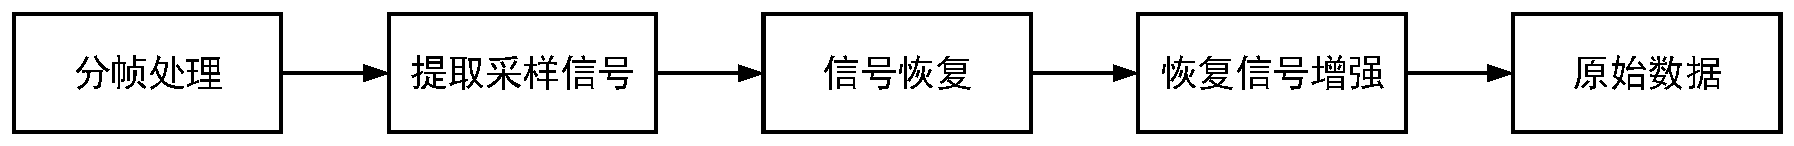
\includegraphics[width=\linewidth]{FIG/SRprocess.pdf}
  \caption{信号恢复流程}
  \label{fig:SRP}
\end{figure*}

\begin{figure*}[!b]
  \centering
  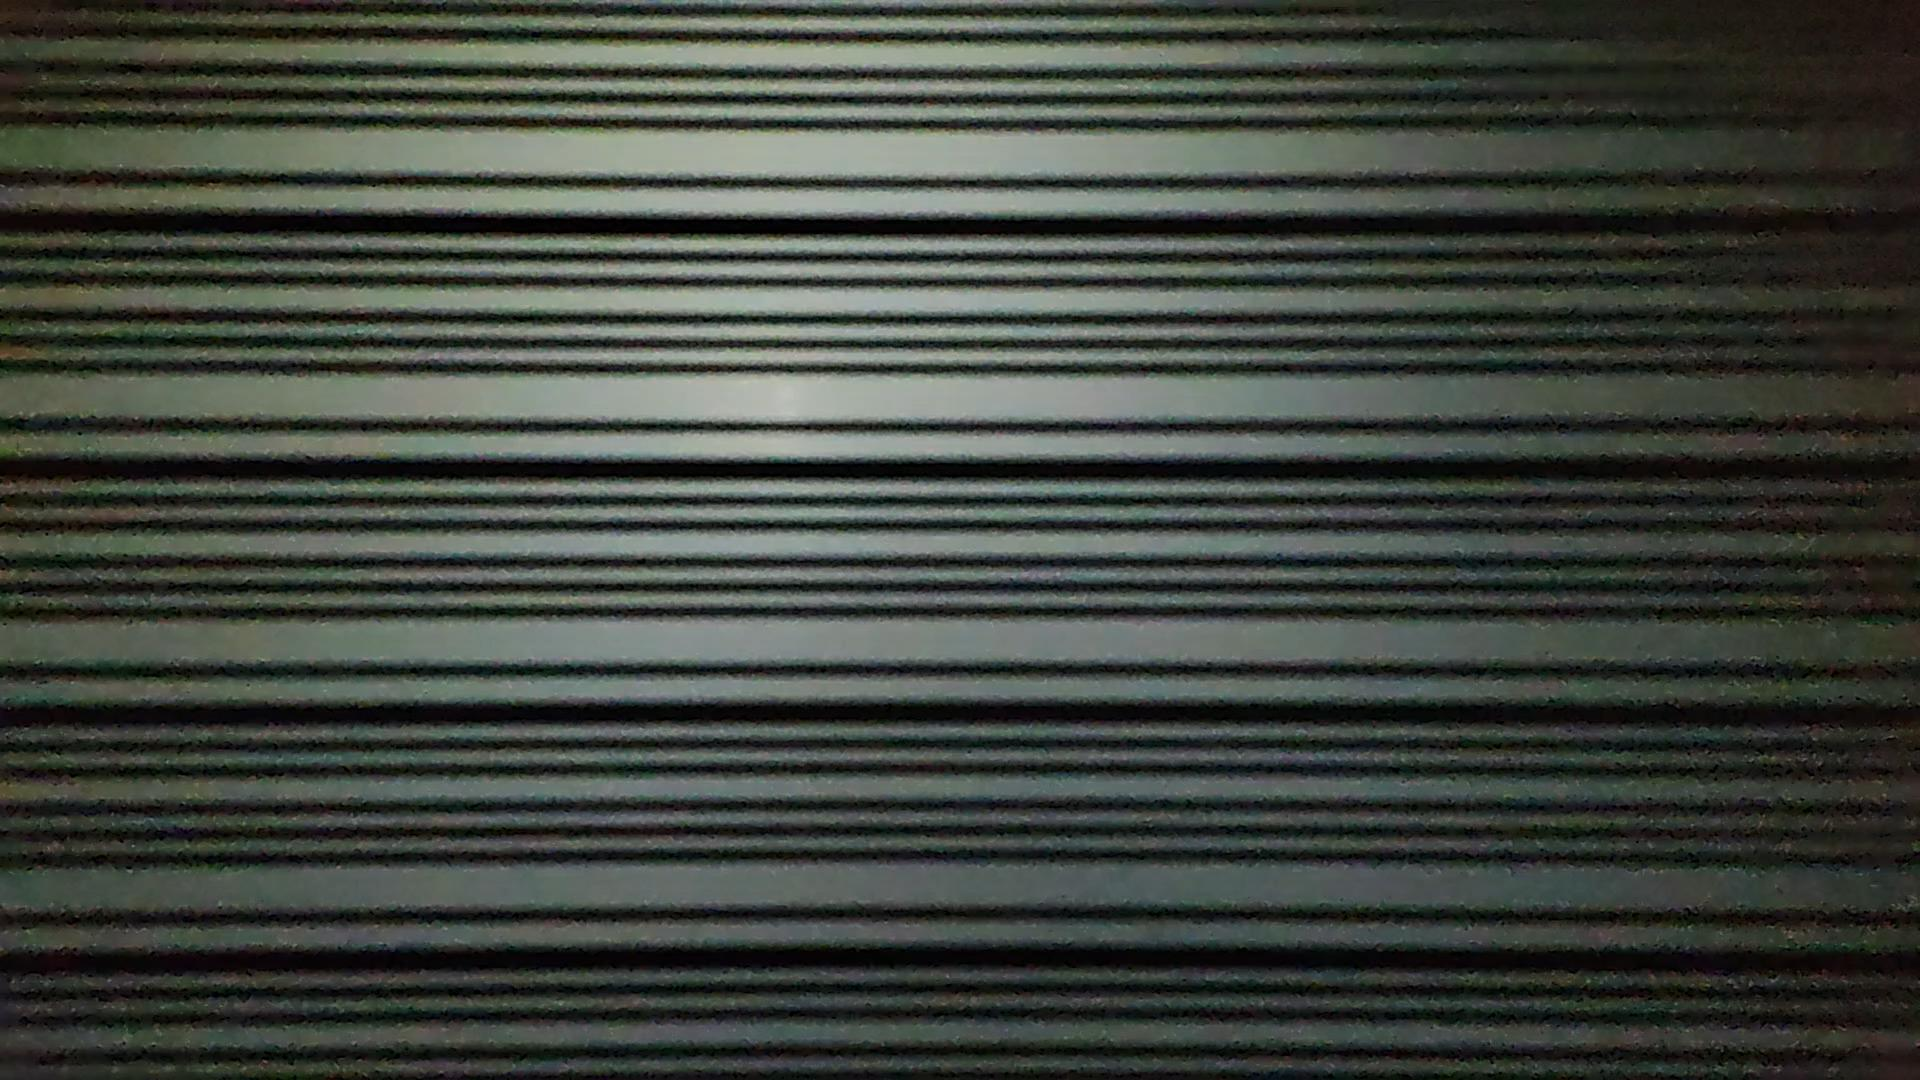
\includegraphics[width=0.7\linewidth]{FIG/stripes.jpg}
  \caption{包含明暗条纹的一帧图像}
  \label{fig:stripes}
\end{figure*}
考虑到上述因素,一帧图像的信号恢复的流程如图\ref{fig:SRP}所示,具体步骤如下:
\begin{enumerate}[topsep = 0 pt, itemsep= 0 pt, parsep=0pt, partopsep=0pt, leftmargin=20pt, itemindent=0pt, labelsep=6pt, label={(\arabic*)}] 

    \item 分帧处理:将视频流通过Matlab分离成一帧帧的图像,如图\ref{fig:stripes}所示。
    \item 提取采样信号:对每一帧图像,调制信号是是关于时间的函数,而采样信号只跟行数有关系。因此,可以通过每一行像素取平均值来过滤随机噪声。最后,每一帧照片将会得到一个一维的离散数组,也是是对应的这一帧图像曝光期间的采样信号,如图\ref{fig:curvefit}所示。


    
    \item 信号恢复:首先,使用加权线性最小二乘和一阶多项式模型的局部回归拟合采样曲线;提取波峰波谷,连续的波峰和波谷之间的中值点作为判定点,连接所有的判定点得到阈值曲线;通过阈值曲线来恢复初始的方波信号,如图\ref{fig:curverecovery}所示。
    \item 波形符号分类:相对于单纯的通过幅值或者宽度来区别信号的类型,本文在这里通过幅值和宽度来共同判别方波信号对应的码元。由于经过曼彻斯特编码之后,两个基本码元的组合类型只有四种,分别是“00, 0, 1, 11”,还有一个标头用“111”表示。通过对方波信号进行归类,如图\ref{fig:curvedata}所示,很容易得到对应的码元组合来恢复初始信号。  
\end{enumerate}

\begin{figure*}[!t]
  \centering
  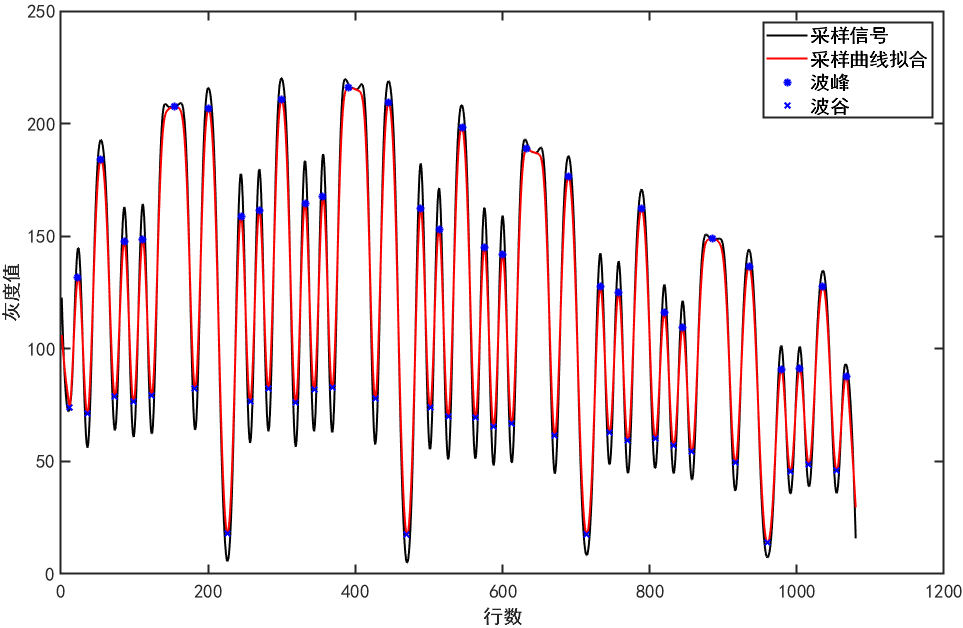
\includegraphics[width=\linewidth]{FIG/samplecurve.png}
  \caption{采样信号的提取和拟合}
  \label{fig:curvefit}
\end{figure*}


\begin{figure*}[!htbp]
  \centering
  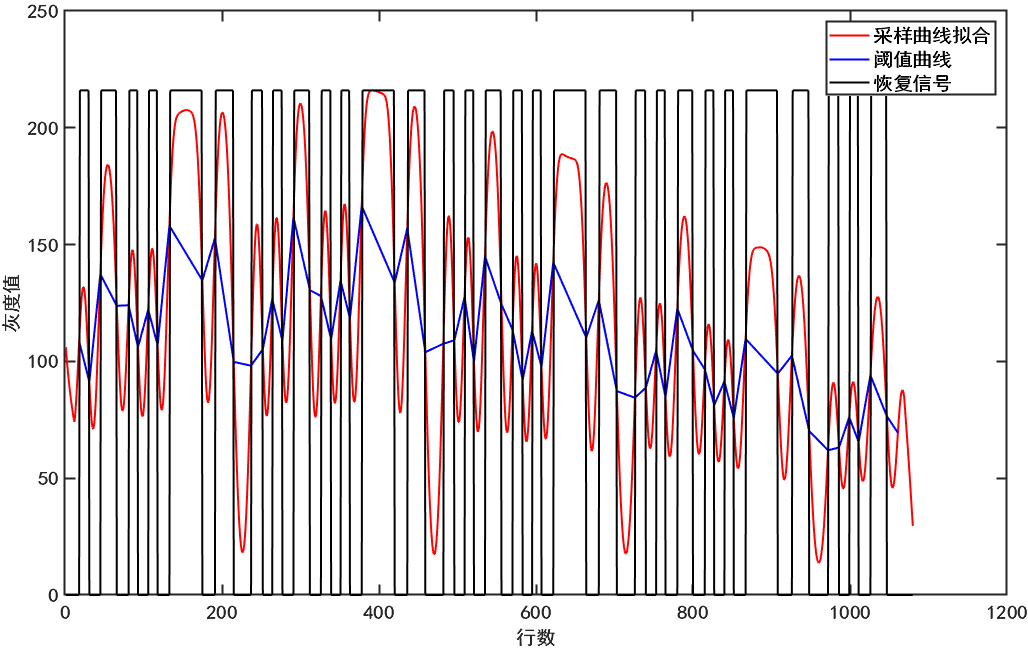
\includegraphics[width=\linewidth]{FIG/signalcurve.png}
  \caption{信号恢复}
  \label{fig:curverecovery}
\end{figure*}


\begin{figure*}[!htbp]
  \centering
  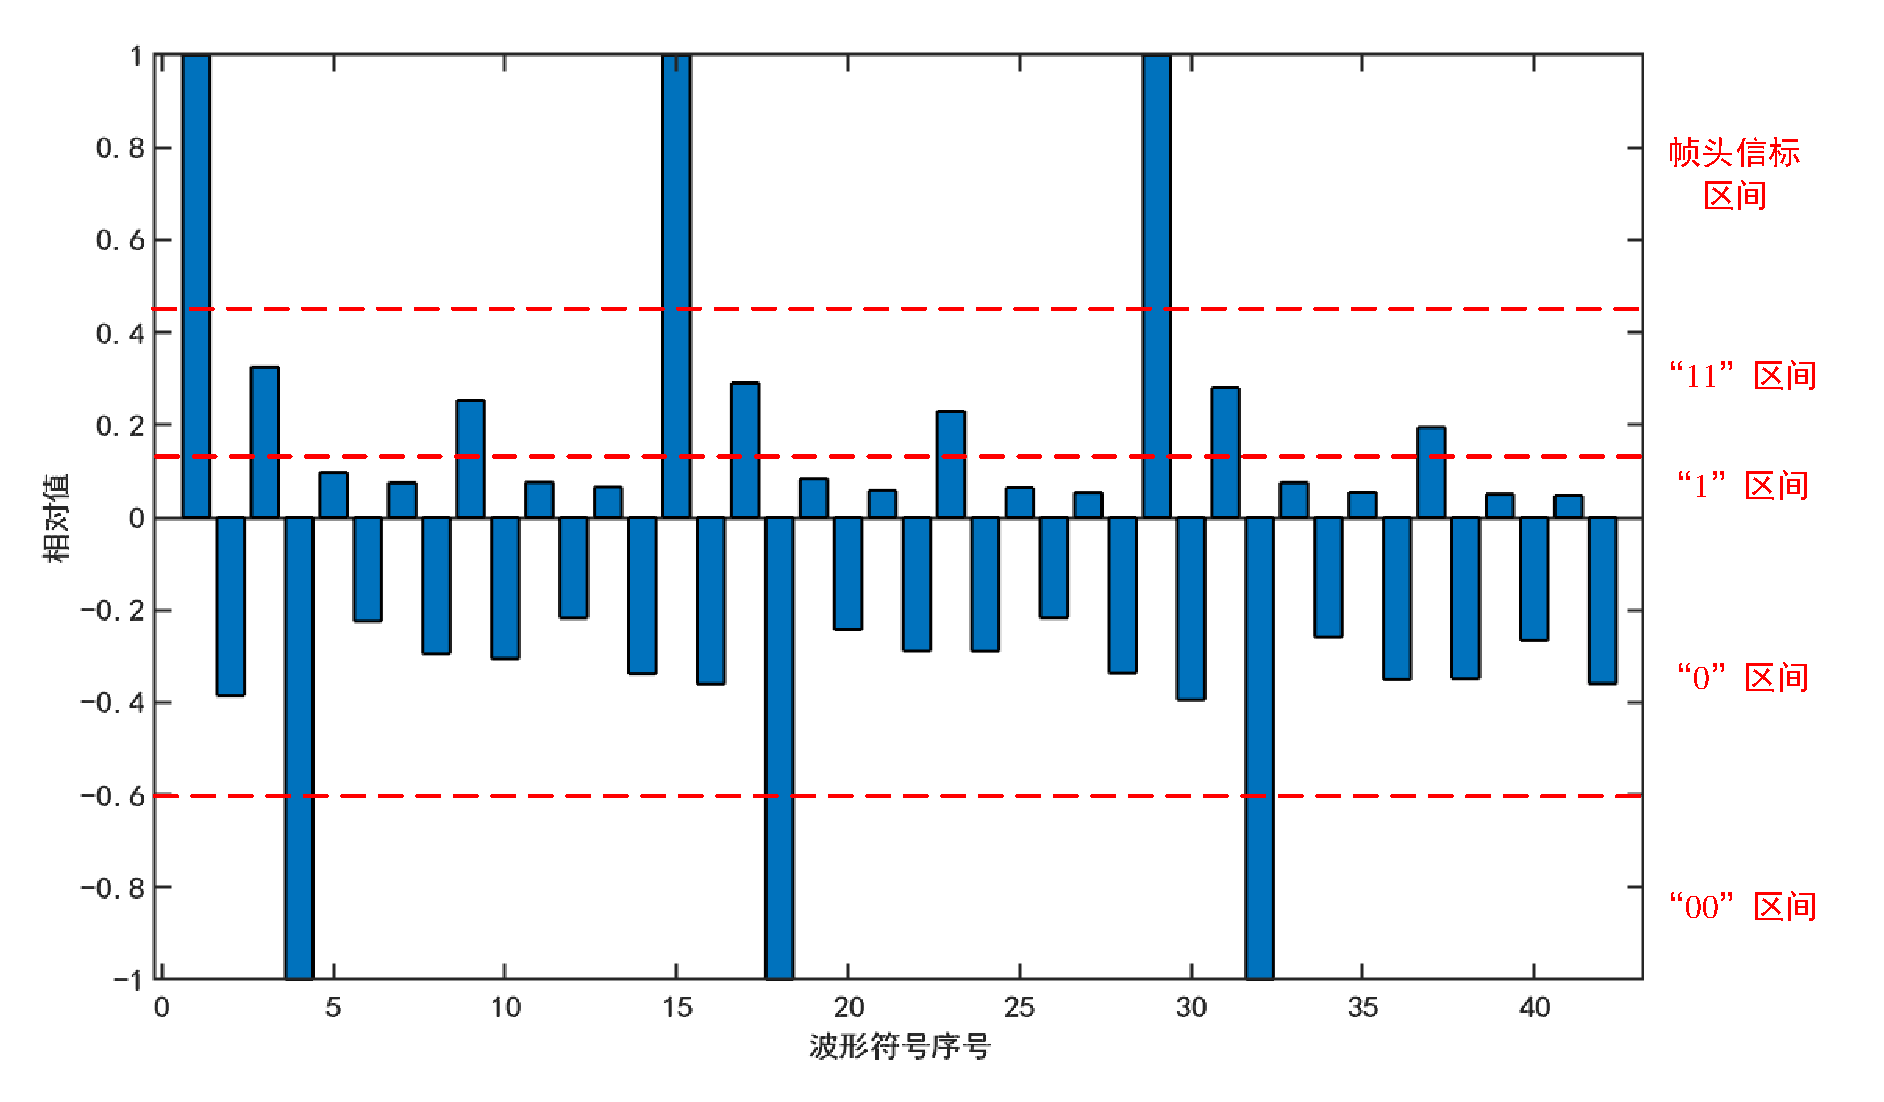
\includegraphics[width=0.9\linewidth]{FIG/curvedata.pdf}
  \caption{波形符号分类}
  \label{fig:curvedata}
\end{figure*}

对连续的每一帧图像进行同样的信号恢复,然后将得到的初始信号拼接在一起,就可以进行连续的信号接收。上述内容给出了一个最简单的基于OOK调制的NLOS OCC系统的设计方案。

\section{系统性能分析}
由于本文所设计的NLOS OCC系统将作为NLOS IS-VLP 系统的一个内嵌模块,其主要的任务是要实现对LED坐标位置的连续准确的接收。因此,对所提出的NLOS OCC系统的性能分析主要考虑两个方面:是否可以克服LOS受阻的问题和信号是否能够准确接收。首先,本系统可以利用反射光进行NLOS OCC,在2.5 m的通信距离下达到0.27kbps,误差率为0。因此可以实现在大部分室内场景下的NLOS通信。其次,本系统考虑到了相机曝光的帧间丢失问题,对每一帧图像至少可以提取到一个完整的信号周期。因此本系统可以达到NLOS IS-VLP 系统的通信要求。


\section{本章小结}
 考虑到NLOS OCC系统的是NLOS IS-VLP系统的一个主要的模块,本章首先推到了NLOS OCC系统的信号恢复模型,给出了信号恢复的理论支持。在此之后,详细的阐述了基于OOK调制的NLOS OCC系统的设计流程,包括硬件系统设计和接收端的信号处理流程以及最后的系统性能分析。

